\documentclass[aspectratio=169]{beamer}

\usepackage{amsmath, amssymb, amsxtra, amsthm, amsfonts}
\usetheme{moloch}
\usecolortheme{beaver}
\setbeamertemplate{footline}
{
  \leavevmode%
  \hbox{%
    \begin{beamercolorbox}[wd=.5\paperwidth,ht=2.25ex,dp=1ex,center]{author in head/foot}%
      \usebeamerfont{author in head/foot}\insertsection
    \end{beamercolorbox}%
    \begin{beamercolorbox}[wd=.5\paperwidth,ht=2.25ex,dp=1ex,right]{date in head/foot}%
      \usebeamerfont{date in head/foot}\inserttitle\hspace*{2em}
      \insertframenumber{} / \inserttotalframenumber\hspace*{2ex}
    \end{beamercolorbox}}%
  \vskip0pt%
}
\makeatother

\usepackage[english]{babel}
\usefonttheme{serif}

\usepackage{mathtools}
\usepackage{graphicx}
\usepackage{bm}
\usepackage{color}
\usepackage[dvipsnames,table]{xcolor}
\usepackage{tikz}
\usepackage{stanli}
\usepackage{verbatim}
\usepackage{tikz}
\usetikzlibrary{shapes,calc,through,3d,patterns}
\usetikzlibrary{decorations.pathreplacing}
\usetikzlibrary{arrows.meta,calc,positioning}

\usepackage{pgfplots}
\usepackage{siunitx} % For formatting numbers
\usepackage{hyperref}
\hypersetup{colorlinks=true,linkcolor=darkred}
\usepackage{multicol}
\usepackage[absolute,overlay,]{textpos}
\usepackage{pgfplots}
\pgfplotsset{width=10cm,compat=1.9}
\usepackage{subcaption}
\usepackage{multirow}
\usepackage{bbding}
\usepackage{arydshln}
\usepackage{mathtools}
\usepackage{tcolorbox}
\usepackage{animate}

\textblockorigin{80mm}{45mm}


\newtheorem{thm}{Theorem}
\newtheorem{cor}[thm]{Corollary}
\newtheorem{prop}[thm]{Proposition}
\newtheorem{lem}[thm]{Lemma}
\theoremstyle{remark}
\newtheorem*{rem}{Remark}

%Block def
\definecolor{darkred}{rgb}{0.6,0,0}
\setbeamertemplate{blocks}[rounded][shadow=false]
\setbeamercolor{block title}{bg=darkred!15,fg=black}
\setbeamercolor{block body}{bg=darkred!5,fg=black}

\setbeamercolor{itemize item}{fg=darkred}
\setbeamercolor{itemize subitem}{fg=darkred}
\setbeamercolor{itemize subsubitem}{fg=darkred}
\setbeamercolor{enumerate item}{fg=darkred}
\setbeamercolor{button}{bg=gray!30,fg=darkred}

\setbeamertemplate{itemize item}[square]
\setbeamertemplate{itemize subitem}[circle]
\setbeamertemplate{itemize subsubitem}[triangle]
\setbeamertemplate{enumerate items}[circle]
\setbeamercolor{item projected}{bg=darkred}

\newcommand{\bolddelta}{\boldsymbol\delta}
\newcommand{\boldxi}{\boldsymbol\xi}
\DeclareMathOperator*{\A}{\text{\raisebox{-0.2cm}{\Huge A}}}




\title{Galerkin and FE approximation}
\subtitle{Linear elastodynamics}
\author{ME473 Dynamic finite element analysis of structures}
\institute{Stefano Burzio}
\date{2025}


\begin{document}
\usenavigationsymbolstemplate{}
{\setbeamertemplate{footline}{}

  \frame{\titlepage
    \begin{tikzpicture}[overlay, remember picture]
      \node[anchor=north east, xshift=-.9cm] at (current page.north east) {
\includegraphics[width=2cm]{../images/epfl_logo.png}};
      \node[anchor=south east, xshift=-.87cm, yshift=.05cm] at (current page.south east)  {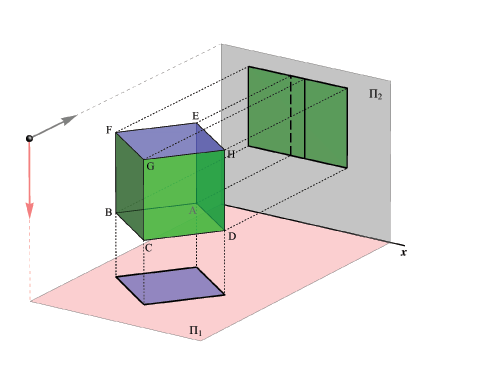
\includegraphics[width=5cm]{../images/projection.png}};
    \end{tikzpicture}
  }

  \begin{frame}{Where do we stand?}
    \begin{center}
      \begin{tabular}{|c|l|l|l|}
        \hline
        \rowcolor{darkred!20}\textbf{Week} & \textbf{Module}                          & \textbf{Lecture topic}  & \textbf{Mini-projects} \\
        \hline
        1                                  & \multirow{2}{7em}{Linear elastodynamics} & Strong and weak forms   &                        \\ \cline{1-1} \cline{3-4}
        2                                  &                                          & Galerkin and FE methods &                        \\ \cline{1-1} \cline{3-4}
        \hline
      \end{tabular}
    \end{center}
    \vspace{1cm}
  \end{frame}

  \begin{frame}
    \textbf{\large Summary}
    \begin{itemize}
      \item Recap week 1
      \item Further evidence in favor of the weak form
      \item Discretisation of the weak form of elastodynamics via Galerkin method
            \begin{itemize}
              \item Example: longitudinal vibration of a bar
              \item Matlab implementation of Galerkin approximation
            \end{itemize}
      \item Finite element method in global coordinate system
    \end{itemize}
    \vspace{.5cm}

    \textbf{\large Recommended readings}
    \begin{enumerate}
      \item Gmür, Dynamique des structures (§2.3, §2.4, §3.1 and §3.2)
      \item Neto et al., Engineering Computation of Structures (§2.1, §2.2 and §2.3)
    \end{enumerate}
  \end{frame}
}

\section{Recap week 1 \\ Strong and weak forms of elastodynamics}
 {\setbeamercolor{background canvas}{bg=darkred!5}
  \setbeamercolor{block body}{bg=darkred!5,fg=black}
  \setbeamercolor{normal text}{fg=black}
  \usebeamercolor[fg]{normal text}

  \begin{frame}{Statement of the linear elastodynamics problem}
    \begin{columns}[T]
      \begin{column}{.65\textwidth}
        \begin{itemize}
          \item \textbf{Object:} \\ A solid $\Omega\subset\mathbb R^{3}$ (beam, shaft, plate etc...) with known material properties: $\mathbf C$ and $\rho$.
                \vspace{0.3cm}
          \item \textbf{Main features:}
                \begin{itemize}
                  \item Acting loads on the body: $\mathbf f$.
                        \vspace{0.1cm}
                  \item Boundary $\Gamma=\Gamma_{u}\cup\Gamma_{\sigma}$ (the surface enclosing the solid).
                        \vspace{0.1cm}
                  \item Boundary conditions: \begin{itemize}
                          \item Prescribed displacements $\mathbf{\hat u}$ on the boundary $\Gamma_{u}$ \item  prescribed loads $\mathbf{\hat f}$ on the boundary on $\Gamma_{\sigma}$.
                                \vspace{0.1cm}
                        \end{itemize}
                  \item Initial displacement $\mathbf u_0$ and initial velocity $\mathbf v_0$ at $t=0$.
                \end{itemize}
        \end{itemize}
      \end{column}
      \hfill
      \begin{column}{.4\textwidth}
        \begin{center}
          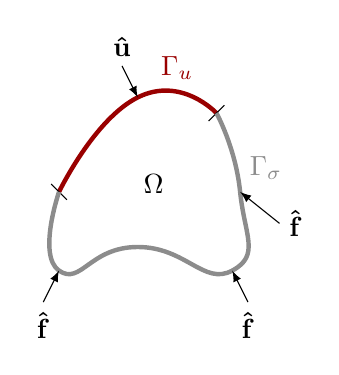
\begin{tikzpicture}
            % Label the region Omega	
            \node at (2.2,2.1) {$\Omega$};
            % Label the boundary Gamma
            \draw[ultra thick, darkred] plot [smooth, tension=1] coordinates {(1,2) (2,3.2) (3,3)};
            \node[darkred, above] at (2.5,3.3) {$\Gamma_u$};
            \draw[thin] (3+0.1,3+0.1) --(3-0.1,3-0.1);
            \draw[thin] (1+0.1,2-0.1) --(1-0.1,2+0.1);
            \draw[latex-]  (2,3.2) --  (2-0.2,3.2+0.4) node[above] {$\mathbf{\hat u}$};
            % Draw part of the boundary Gamma_sigma
            \draw[ultra thick, gray!90] plot [smooth, tension=1] coordinates {(3,3) (3.3,2) (3.2,1) (2,1.3) (1,1) (1,2)};
            \node[gray!90, right] at (3.3,2.3) {$\Gamma_\sigma$};
            \draw[latex-]  (1,1) --  (1-0.2,1-0.4) node[below] {$\mathbf{\hat f}$};;
            \draw[latex-]  (3.2,1) --  (3.2+0.2,1-0.4) node[below] {$\mathbf{\hat f}$};
            \draw[latex-]  (3.3,2) --  (3.3+0.5,2-0.4) node[right] {$\mathbf{\hat f}$};
          \end{tikzpicture}
        \end{center}
      \end{column}
    \end{columns}
  \end{frame}


  \begin{frame}{Statement of the linear elastodynamics problem}
    \begin{itemize}
      \item \textbf{Unknown:} displacement $\mathbf u(\mathbf x,t)\in \mathbb R^{3}$
    \end{itemize}
    \vspace{-0.3cm}
    \begin{columns}[T]
      \begin{column}{.5\textwidth}
        \begin{center}
          \textbf{Undeformed solid}
          \vspace{0.5cm}
          \newline
          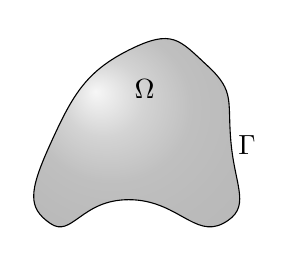
\begin{tikzpicture}
            % Draw the potato-like shape
            \shade [ball color= gray!50!black, opacity=.3] plot [thick,smooth cycle, tension=1] coordinates  {(1,2) (2,3.2) (3,3) (3.3,2) (3.2,1) (2,1.3) (1,1)};
            \draw plot [thick,smooth cycle, tension=1] coordinates {(1,2) (2,3.2) (3,3) (3.3,2) (3.2,1) (2,1.3) (1,1)};
            % Label the region Omega	
            \node at (2.2,2.7) {$\Omega$};
            % Label the boundary Gamma
            \node at (3.5,2) {$\Gamma$};
          \end{tikzpicture}
        \end{center}
      \end{column}
      \hfill
      \begin{column}{.5\textwidth}
        \begin{center}
          \textbf{Deformed solid}
          \vspace{0.5cm}
          \newline
          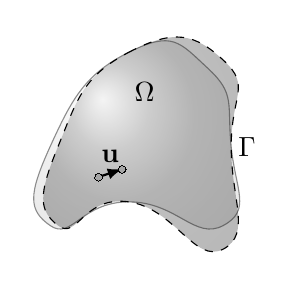
\begin{tikzpicture}
            % Draw the potato-like shape
            \shade [ball color= gray!90, opacity=.1] plot [thick,smooth cycle, tension=1] coordinates  {(1,2) (2,3.2) (3,3) (3.3,2) (3.2,1) (2,1.3) (1,1)};
            \draw[color=gray!90] plot [opacity=.1,smooth cycle, tension=1] coordinates {(1,2) (2,3.2) (3,3) (3.3,2) (3.2,1) (2,1.3) (1,1)};
            \shade [ball color= gray!50!black, opacity=.3] plot [thick,smooth cycle, tension=1] coordinates  {(1.1,2) (2,3.2) (3.2,3.1) (3.3,2) (3.2,0.7) (2,1.3) (1.1,1)};
            \draw[dashed] plot [color=gray!40!black, opacity=.3,thick, smooth cycle, tension=1] coordinates {(1.1,2) (2,3.2) (3.2,3.1) (3.3,2) (3.2,0.7) (2,1.3) (1.1,1)};
            % Label the region Omega	
            \node at (2.2,2.7) {$\Omega$};
            % Label the boundary Gamma
            \node at (3.5,2) {$\Gamma$};
            \draw[thick,-latex] (2,2,1) to node[midway,above]{$\mathbf u$} (2.3,2.1,1);
            \node[draw,shape=circle,fill=black!35,minimum size=1mm,line width=0mm,inner sep=0] at (2,2,1) {};
            \node[draw,shape=circle,fill=black!35,minimum size=1mm,line width=0mm,inner sep=0] at (2.3,2.1,1) {};
          \end{tikzpicture}
        \end{center}
      \end{column}
    \end{columns}
    \begin{itemize}
      \item PDE governing the evolution of the displacements $\mathbf u$:
            $$\boldsymbol\nabla^T\mathbf C\boldsymbol\nabla \mathbf u(\mathbf x,t)+\mathbf f(\mathbf x,t)=\rho\mathbf{\ddot{u}}(\mathbf x,t) \qquad \forall (\mathbf x,t)\in\Omega\times]0,T[$$
    \end{itemize}
  \end{frame}


  \begin{frame}{Strong and weak forms of elastodynamics}
    \vspace{-0.5cm}
    \begin{center}
      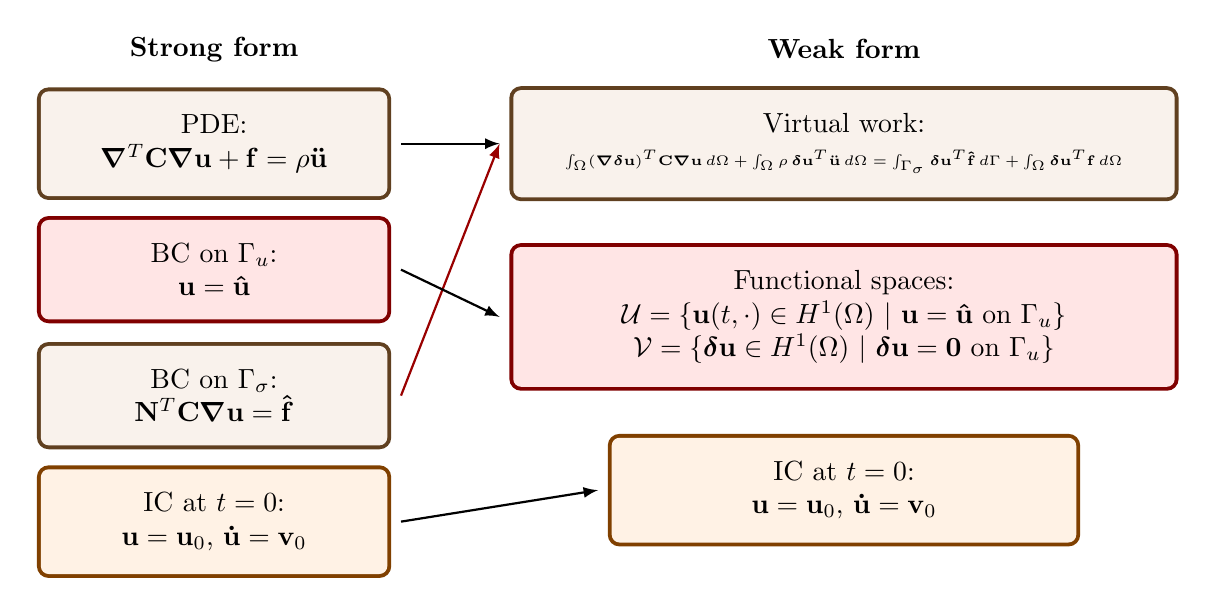
\begin{tikzpicture}[scale=0.8]
        \node (sf) at (-2,6.5) {
          \centering \textbf{Strong form}
        };
        \node (wf) at (8,6.5) {
          \centering \textbf{Weak form}
        };
        \node (pde) at (-2,5) {
          \begin{tcolorbox}[colframe=brown!50!black, colback=brown!10, coltitle=black, rounded corners, width=4.5cm]
            \centering PDE: \\ $\boldsymbol\nabla^T\mathbf C\boldsymbol\nabla \mathbf u+\mathbf f=\rho\mathbf{\ddot{u}}$
          \end{tcolorbox}
        };
        \node (bc1) at (-2,3) {
          \begin{tcolorbox}[colframe=red!50!black, colback=red!10, coltitle=black, rounded corners,width=4.5cm]
            \centering BC on $\Gamma_u$: \\ $\mathbf u=\mathbf{\hat u}$
          \end{tcolorbox}
        };
        \node (bc2) at (-2,1) {
          \begin{tcolorbox}[colframe=brown!50!black, colback=brown!10, coltitle=black, rounded corners,width=4.5cm]
            \centering BC on $\Gamma_\sigma$: \\ $\mathbf N^T\mathbf  C\boldsymbol\nabla\mathbf  u=\mathbf{\hat f}$
          \end{tcolorbox}
        };

        \node (ic1) at (-2,-1) {
          \begin{tcolorbox}[colframe=orange!50!black, colback=orange!10, coltitle=black, rounded corners,width=4.5cm]
            \centering IC at $t=0$: \\ $\mathbf{u}=\mathbf u_0$, $\mathbf{\dot u}=\mathbf v_0$
          \end{tcolorbox}
        };
        \node (inteq) at (8,5) {
          \begin{tcolorbox}[colframe=brown!50!black, colback=brown!10, coltitle=black, rounded corners, width=8.5cm]
            \centering Virtual work: \\\vspace{0.2cm} \tiny $\int_\Omega (\boldsymbol\nabla \bolddelta\mathbf u)^{T} \mathbf C\boldsymbol\nabla \mathbf u\, d\Omega+\int_\Omega\rho\, \bolddelta\mathbf u^{T}\mathbf{\ddot{u}}\, d\Omega=\int_{\Gamma_\sigma} \bolddelta\mathbf u^{T}\mathbf{\hat f} \, d\Gamma+\int_\Omega \bolddelta\mathbf u^{T}\mathbf f\, d\Omega$
          \end{tcolorbox}
        };
        \node (funcsp) at (8,2.25) {
          \begin{tcolorbox}[colframe=red!50!black, colback=red!10, coltitle=black, rounded corners,width=8.5cm]
            \centering Functional spaces: \\ $ \mathcal U =\{\mathbf u(t,\cdot)\in H^1(\Omega)\ |\ \mathbf u=\mathbf{\hat u}\ \mbox{on}\ \Gamma_u\}$ \\
            $ \mathcal V =\{\bolddelta\mathbf u\in H^1(\Omega)\ |\ \bolddelta\mathbf u=\mathbf 0\ \mbox{on}\ \Gamma_u\}$
          \end{tcolorbox}
        };
        \node (ic2) at (8,-0.5) {
          \begin{tcolorbox}[colframe=orange!50!black, colback=orange!10, coltitle=black, rounded corners,width=6cm]
            \centering IC at $t=0$: \\ $\mathbf{u}=\mathbf u_0$, $\mathbf{\dot u}=\mathbf v_0$
          \end{tcolorbox}
        };
        % Drawing arrows
        \draw[-latex, thick] (pde.east) -- (inteq.west);
        \draw[-latex, thick, darkred] (bc2.east) -- (inteq.west);
        \draw[-latex, thick] (bc1.east) -- (funcsp.west);
        \draw[-latex, thick] (ic1.east) -- (ic2.west);
      \end{tikzpicture}
    \end{center}
  \end{frame}

  \begin{frame}{Strong form for longitudinal vibrations of a bar}
    \begin{columns}
      \column{0.65\textwidth}
      \begin{center}
        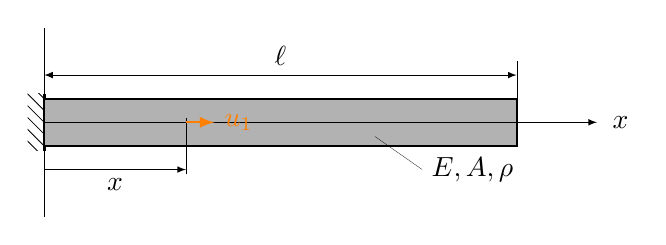
\begin{tikzpicture}[scale=0.6]
          \point{a}{0}{0};
          \support {3}{a}[270];

          % Draw the rectangle
          \filldraw[fill=gray!60, draw=black,thick] (0,-0.5) rectangle (10,0.5);

          %axis
          \draw[-latex, ultra thin] (0,0) -- (11.7,0);
          \draw[ ultra thin] (0,-2) -- (0,2);
          \node at (12.2,0) {\(x\)};
          % displacement 
          \draw[-latex,ultra thin] (0,-1) to node[midway,below] {$x$} (3,-1);
          \draw[ultra thin] (3,-1.1) -- (3,0.1);
          \draw[-latex,thick,orange] (3,0) to  (3.6,0) node[right]{$u_{1}$};
          % length
          \draw[ultra thin] (10,0) -- (10, 1.3) ;
          \draw[latex-latex, ultra thin]  (0,1)  to node[sloped,midway,above] {$\ell$}(10,1) ;
          \draw[ultra thin]  (7,-0.3) -- (8,-1) node[right]{$E,A,\rho$};
        \end{tikzpicture}
      \end{center}

      \column{0.5\textwidth}
      {\tiny \begin{itemize}
          \item $A$ cross-sectional area
          \item $\ell$ length
          \item $E$ Young's modulus (isotropic bar)
          \item $\rho$ material density
          \item $u_1$ axial displacement
          \item $x$ axial coordinate
        \end{itemize}}

    \end{columns}

    \vspace{0.3cm}
    \begin{block}{}
      Find $u_{1}\in C^2([0,\ell]\times[0,T])$ such that
      \[
        EA \partial^{2}_{xx}u_{1}(x, t) = \rho A \ddot{u}_1(x, t)
      \]
      \begin{multicols}{2}
        \textbf{boundary conditions:}
        \[
          \begin{aligned}
             & \textcolor{darkred}{u_1(0, t) = 0}                  \\
             & \textcolor{brown}{EA \partial_{x} u_1(\ell, t) = 0} \\
          \end{aligned}
        \]

        \textbf{initial conditions:}
        \[
          \begin{aligned}
             & u_1(x, 0) =  u_0(x)      \\
             & \dot{u}_1(x, 0) = v_0(x) \\
          \end{aligned}
        \]
      \end{multicols}
      \vspace{0.01cm}
    \end{block}
  \end{frame}



  \begin{frame}{Weak form for longitudinal vibrations of a bar}
    \begin{block}{}
      Find the displacement$u_{1}\in \mathcal U$ such that for any virtual displacement $\delta u_1\in\mathcal V$ we have
      \[
        \int_0^\ell EA\, \partial_{x} u_1\,\partial_{x}(\delta u_1)\ dx +\int_0^\ell\rho A \ddot{u}_1\delta u_1\, dx=0,
      \]
      where
      \begin{align*}
        \mathcal U & =\big\{u_{1}(\cdot,t)\in H^1(]0,\ell[)\ |\   {\color{darkred}u_1(0,t)=0}\ \forall t\in]0,T[\big\} \\
        \mathcal V & =\big\{\delta u_{1}\in H^1(]0,\ell[)\ |\  {\color{darkred}\delta u_{1}(0)=0}\big\}
      \end{align*}
    \end{block}
    Moreover, the initial conditions read
    $$\begin{aligned}
        u_1(x,0)      & = u_0(x), \\
        \dot u_1(x,0) & = v_0(x).
      \end{aligned}$$
  \end{frame}
 }

\section{Further evidence in favor of the weak form}

\begin{frame}{Weighted residuals}
  \begin{itemize}
    \item  Let $\mathbf u$ be a solution of
          $$\boldsymbol\nabla^T\mathbf C\boldsymbol\nabla \mathbf u+\mathbf f-\rho\mathbf{\ddot{u}}=0.$$
    \item Let $\mathbf u^{h}$ an approximate solution.
          \begin{block}{}
            In general $\mathbf u^{h}$ does not satisfy the differential equation and hence results in an error or a \emph{residual}:
            $$\boldsymbol\nabla^T\mathbf C\boldsymbol\nabla \mathbf u^{h}+\mathbf f-\rho\mathbf{\ddot{u}}^{h}=\mathbf R^{h}.$$
          \end{block}
    \item We impose that the residual is zero in a certain Euclidean vector space $\mathcal V^h$ of finite dimension. Thus
          $$\langle\mathbf R^{h}, \mathbf v^h\rangle=0\qquad \text{for all }\mathbf v^h\in\mathcal V^{h}$$
          where $\langle\cdot,\cdot\rangle$ denotes the scalar product.
  \end{itemize}
\end{frame}

\begin{frame}{Weighted residual}
  \begin{itemize}
    \item For vector-valued functions, there is a natural definition of scalar product:
          $$\langle\mathbf f,\mathbf g\rangle=\int_{\Omega}\mathbf f^{T}\mathbf g\, d\Omega.$$
    \item Hence $\langle\mathbf R^{h}, \mathbf v^h\rangle=0$  for all $\mathbf v^h\in\mathcal V^{h}$ implies
          $$\int_{\Omega}(\mathbf v^h)^{T}\big(\boldsymbol\nabla^T\mathbf C\boldsymbol\nabla \mathbf u^h+\mathbf f-\rho\mathbf{\ddot{u}}^h\big)\, d\Omega=0 \qquad \text{for all }\mathbf v^h\in\mathcal V^{h}.$$
    \item Applying the divergence theorem results into the equation of the weak form:
          $$\int_\Omega (\boldsymbol\nabla \mathbf v^h)^{T} \mathbf C\boldsymbol\nabla \mathbf u^h\, d\Omega+\int_\Omega\rho(\mathbf v^h)^{T}\mathbf{\ddot{u}}^h\, d\Omega=\int_{\Gamma_\sigma} (\mathbf v^h)^{T}\mathbf{\hat f} \, d\Gamma+\int_\Omega (\mathbf v^h)^{T}\mathbf f\, d\Omega \qquad \forall\mathbf v^h\in\mathcal V^{h}.$$
  \end{itemize}
\end{frame}

\begin{frame}{Hamilton's principle - principle of stationary action}
  \begin{columns}[T]
    \begin{column}{.6\textwidth}
      The path taken by the system is defined by the admissible function $\mathbf{u}$  that makes the functional stationary:
      $$J=\int_{t_{1}}^{t_{2}}T(\mathbf{\dot u})-U(\mathbf{u})+W(\mathbf{u})\, dt.$$
      \begin{itemize}
        \item T is the total kinetic energy,
        \item U represents the potential (elastic) energy of the flexible structure,
        \item W the work done by external loads that are acting on the body.
      \end{itemize}
    \end{column}
    \hfill
    \begin{column}{.4\textwidth}
      \begin{center}
        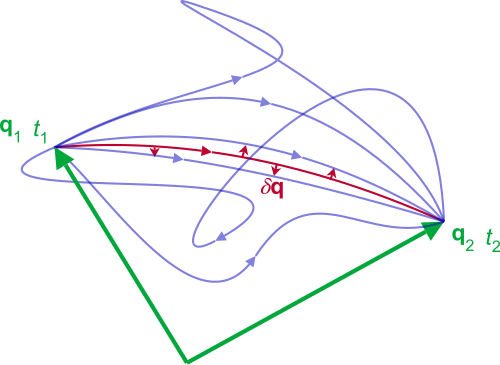
\includegraphics[scale=0.3]{../images/Least_action_principle.png}
        \noindent{\tiny\emph{Credit: Wikipedia - Hamilton's principle}}
      \end{center}
    \end{column}
  \end{columns}
\end{frame}

\begin{frame}{Hamilton's principle - principle of stationary action.}
  \begin{itemize}
    \item The kinetic energy associated with a flexible body that has volume $\Omega$ is given as
          $$T(\mathbf{\dot u})=\frac{1}{2}\int_{\Omega}\rho \mathbf{\dot u}^{T}\mathbf{\dot u}\, d\Omega$$
    \item The total elastic energy of a deformable structure is given as
          $$U(\mathbf{u})=\frac{1}{2}\int_{\Omega}\bm \varepsilon ^{T}\mathbf C\bm{\varepsilon}\, d\Omega=\frac{1}{2}\int_\Omega (\boldsymbol\nabla \mathbf u)^{T} \mathbf C\boldsymbol\nabla \mathbf u\, d\Omega$$
          where $\bm{\varepsilon}$ is the elastic strain and $\mathbf C$ is the stiffness material matrix.
    \item The total work W done by the external mechanical loading is given by
          $$W(\mathbf{u})=\int_{\Omega}\mathbf u ^{T}\mathbf f\, d\Omega+\int_{\Gamma_\sigma} \mathbf u^{T}\mathbf{\hat f} \, d\Gamma$$
  \end{itemize}
\end{frame}

\begin{frame}{Hamilton's principle}
  \begin{itemize}
    \item Computing the first variation $\delta J$, and imposing $\delta J=0$, yields to:
          $$\int_{t_{1}}^{t_{2}}\Big[\int_\Omega-\rho(\bolddelta\mathbf u)^{T}\mathbf{\ddot{u}}\, d\Omega-(\bolddelta \bm\varepsilon)^{T} \mathbf C\bm\varepsilon+(\bolddelta\mathbf u)^{T}\mathbf f\, d\Omega+\int_{\Gamma_\sigma} (\bolddelta\mathbf u)^{T}\mathbf{\hat f} \, d\Gamma \Big]\, dt=0$$
          for every virtual displacement $\bolddelta\mathbf u$ which satisfies $\bolddelta\mathbf u=0$ on $\Gamma_{u}$.
    \item This implies the weak form of elastodynamics:
          $$\int_\Omega (\boldsymbol\nabla \bolddelta\mathbf u)^{T} \mathbf C\boldsymbol\nabla \mathbf u\, d\Omega+\int_\Omega\rho(\bolddelta\mathbf u)^{T}\mathbf{\ddot{u}}\, d\Omega=\int_{\Gamma_\sigma} (\bolddelta\mathbf u)^{T}\mathbf{\hat f} \, d\Gamma+\int_\Omega (%
            \bolddelta\mathbf u)^{T}\mathbf f\, d\Omega \qquad \forall\bolddelta\mathbf u.$$
  \end{itemize}
\end{frame}

\begin{frame}{Weak form: a cornerstone concept}
  \vspace{-0.5cm}
  \begin{center}
    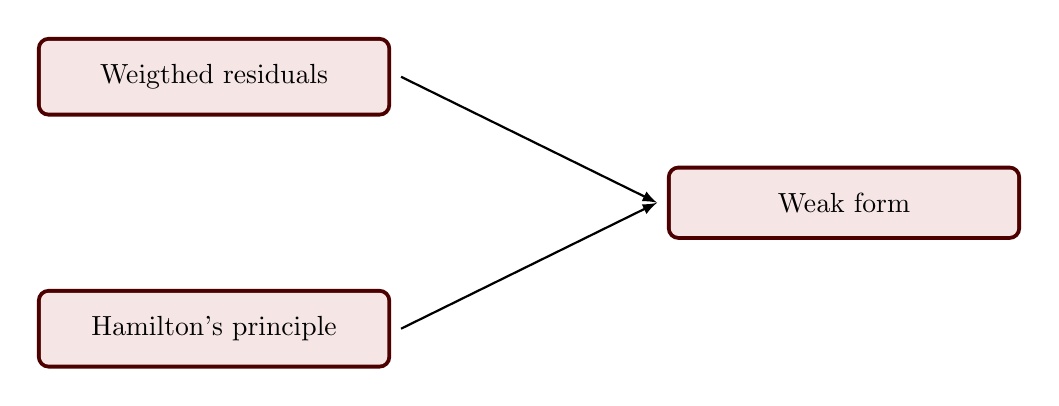
\begin{tikzpicture}[scale=0.8]
      \node (wr) at (-2,2) {
        \begin{tcolorbox}[colframe=darkred!50!black, colback=darkred!10, coltitle=black, rounded corners, width=4.5cm]
          \centering Weigthed residuals
        \end{tcolorbox}
      };
      \node (hp) at (-2,-2) {
        \begin{tcolorbox}[colframe=darkred!50!black, colback=darkred!10, coltitle=black, rounded corners,width=4.5cm]
          \centering Hamilton's principle
        \end{tcolorbox}
      };
      \node (wf) at (8,0) {
        \begin{tcolorbox}[colframe=darkred!50!black, colback=darkred!10, coltitle=black, rounded corners, width=4.5cm]
          \centering Weak form
        \end{tcolorbox}
      };
      % Drawing arrows
      \draw[-latex, thick] (wr.east) -- (wf.west);
      \draw[-latex, thick] (hp.east) -- (wf.west);
    \end{tikzpicture}
  \end{center}
\end{frame}

\section{Galerkin method}

\begin{frame}{General ideas of Galerkin methods}
  \begin{columns}[T]
    \begin{column}{.68\textwidth}\vspace{1.2cm}
      \vspace{-1cm}
      \begin{center}
        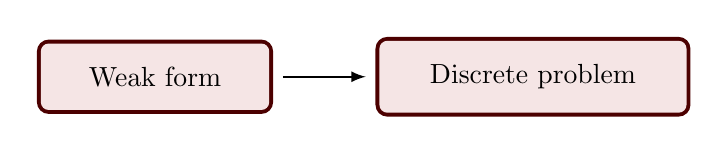
\begin{tikzpicture}[scale=0.8]
          \node (wr) at (-2,0) {
            \begin{tcolorbox}[colframe=darkred!50!black, colback=darkred!10, coltitle=black, rounded corners, width=3cm]
              \centering Weak form
            \end{tcolorbox}
          };
          \node (dp) at (4,0) {
            \begin{tcolorbox}[colframe=darkred!50!black, colback=darkred!10, coltitle=black, rounded corners, width=4cm]
              \centering Discrete problem
            \end{tcolorbox}
          };
          % Drawing arrows
          \draw[-latex, thick] (wr.east) -- (dp.west);
        \end{tikzpicture}
      \end{center}

      \begin{itemize}
        \item Galerkin methods are a class of numerical techniques used to transform differential equations in weak formulation, into discrete problems.
        \item The approximate solution is determined via a finite set of \textbf{basis functions}.
        \item Galerkin approximation compute the best possible approximate solution among a family of potential solutions.
      \end{itemize}

    \end{column}
    \hfill
    \begin{column}{.28\textwidth}
      \begin{center}
        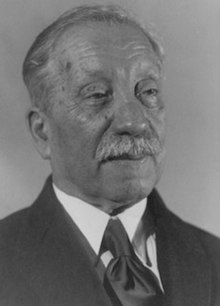
\includegraphics[scale=0.5]{../images/Galerkin}

        \noindent{\tiny\emph{Boris Galerkin 1871 - 1945}}
      \end{center}
    \end{column}
  \end{columns}
\end{frame}

\begin{frame}{Approximate solution of the weak form}
  \textbf{\large Finite-dimensional functional spaces}
  \newline\noindent Choose subspaces $\mathcal U^{h}\subset \mathcal U$ and $\mathcal V^{h}\subset \mathcal V$ of {\color{darkred}dimension $n$}  and solve the \emph{projected weak form} into such subspaces. Moreover, we impose $\mathcal U^{h}=\mathcal V^{h}$.
  \vspace{0.1cm}
  \begin{block}{\large Displacement approximation}
    Instead of searching for $\mathbf u\in \mathcal U$ such that the weak form is satisfied for any $\bolddelta \mathbf u\in \mathcal V$, we shall search for $\mathbf u^{h}\in\mathcal U^{h}$ such that the weak form is satisfied for any $\bolddelta \mathbf u^{h}\in \mathcal V^{h}$.
    \begin{align*}
       & \mathbf u(\mathbf x,t)\approx\mathbf u^{h}(\mathbf x,t)\in\mathcal U^{h}\subset\mathcal U                 \\
       & \bolddelta\mathbf u(\mathbf x)\approx\bolddelta\mathbf u^{h}(\mathbf x)\in\mathcal V^{h}\subset\mathcal V
    \end{align*}
  \end{block}
  \vspace{0.1cm}

  The key property of the Galerkin approach is that the error is \emph{orthogonal} to the chosen subspaces.
\end{frame}

{\setbeamercolor{background canvas}{bg=darkred!5}
\setbeamercolor{block body}{bg=darkred!5,fg=black}

\begin{frame}{Shape functions}
  Let {\color{darkred}$\mathbf u^{h}(\mathbf x,t)=\mathbf H(\mathbf x)\mathbf q(t)$} and {\color{orange}$\bolddelta\mathbf u^{h}(\mathbf x)=\mathbf H(\mathbf x)\bolddelta\mathbf q$} where
  \begin{itemize}
    \item $\mathbf H(\mathbf x)$ is a $3\times n$ matrix of \textbf{shape functions}, defined \emph{globally} on $\Omega$.
    \item $\mathbf q(t)$ is a $n\times 1$ vector of (\emph{unknown}) time-dependent functions.
    \item $\bolddelta \mathbf q$ is a $n\times 1$ vector of constants.
  \end{itemize}
  Shape functions are linearly independent: they form a basis of $\mathcal U^h=\mathcal V^h$.
    {\footnotesize
      \begin{block}{}
        $$
          \begin{pmatrix}
            u_{1}^{h}(\mathbf x,t) \\
            u_{2}^{h}(\mathbf x,t) \\
            u_{3}^{h}(\mathbf x,t) \\
          \end{pmatrix}
          =
          \begin{bmatrix}
            h_{11}(\mathbf x) & h_{12}(\mathbf x) & \dots & h_{1n}(\mathbf x) \\
            h_{21}(\mathbf x) & h_{22}(\mathbf x) & \dots & h_{2n}(\mathbf x) \\
            h_{31}(\mathbf x) & h_{32}(\mathbf x) & \dots & h_{3n}(\mathbf x) \\
          \end{bmatrix}
          \begin{pmatrix}
            q_{1}(t) \\
            q_{2}(t) \\
            \vdots   \\
            q_{n}(t)
          \end{pmatrix}
        $$

        $$
          \begin{pmatrix}
            \delta u_{1}^{h}(\mathbf x) \\
            \delta u_{2}^{h}(\mathbf x) \\
            \delta u_{3}^{h}(\mathbf x) \\
          \end{pmatrix}
          =
          \begin{bmatrix}
            h_{11}(\mathbf x) & h_{12}(\mathbf x) & \dots & h_{1n}(\mathbf x) \\
            h_{21}(\mathbf x) & h_{22}(\mathbf x) & \dots & h_{2n}(\mathbf x) \\
            h_{31}(\mathbf x) & h_{32}(\mathbf x) & \dots & h_{3n}(\mathbf x) \\
          \end{bmatrix}
          \begin{pmatrix}
            \delta  q_{1} \\
            \delta q_{2}  \\
            \vdots        \\
            \delta  q_{n}
          \end{pmatrix}
        $$
      \end{block}
    }
\end{frame}
}

\begin{frame}{Approximate solution of the weak form}
  \begin{itemize}
    \item Find ${\color{darkred}\mathbf u^{h}}\in\mathcal U^{h}$ such that for all ${\color{orange}\bolddelta\mathbf u^{h}}\in\mathcal V^{h}$ we have
          $$\int_{\Omega} (\boldsymbol\nabla {\color{orange}\bolddelta\mathbf u^{h}} )^{T} \mathbf C\boldsymbol\nabla {\color{darkred}\mathbf u^{h}}\, d\Omega+\int_{\Omega} \rho({\color{orange}\bolddelta\mathbf u^{h}})^{T}{\color{darkred}\mathbf{\ddot{u}}^{h}}\, d\Omega=\int_{\Gamma_\sigma} ({\color{orange}\bolddelta\mathbf u^{h}})^{T}\mathbf{\hat f} \, d\Gamma+\int_{\Omega}  ({\color{orange}\bolddelta\mathbf u^{h}})^{T}\mathbf f\, d\Omega$$
    \item   Find ${\color{darkred}\mathbf q(t)}\in\mathbb R^{n}$ such that for all ${\color{orange}\bolddelta\mathbf q}\in\mathbb R^{n}$ we have
          $$\int_{\Omega} (\boldsymbol\nabla{\color{orange} \mathbf H\bolddelta\mathbf q})^{T} \mathbf C\boldsymbol\nabla {\color{darkred}\mathbf H\mathbf q(t)}\, d\Omega+\int_{\Omega} \rho( {\color{orange}\mathbf H\bolddelta\mathbf q})^{T} {\color{darkred}\mathbf H\mathbf{\ddot{q}}(t)}\, d\Omega=\int_{\Gamma_\sigma} ({\color{orange}\mathbf H\bolddelta\mathbf q})^{T}\mathbf{\hat f} \, d\Gamma+\int_{\Omega}  ({\color{orange}\mathbf H\bolddelta\mathbf q})^{T}\mathbf f\, d\Omega$$
    \item  Rearranging the terms we obtain the following expression:
          {\small $${\color{orange}\bolddelta\mathbf q}^{T}\Big[\Big(\underbrace{\int_{\Omega} (\boldsymbol\nabla {\color{orange}\mathbf H})^{T} \mathbf C\boldsymbol\nabla {\color{darkred}\mathbf H}\, d\Omega}_\text{$\mathbf K$}\Big) {\color{darkred}\mathbf q(t)}+\Big(\underbrace{\int_{\Omega} \rho\, {\color{orange}\mathbf H}^{T} {\color{darkred}\mathbf H}\, d\Omega}_\text{$\mathbf M$}\Big) {\color{darkred}\mathbf{\ddot{q}}(t)}-\Big(\underbrace{\int_{\Gamma_\sigma} {\color{orange}\mathbf H}^{T}\mathbf{\hat f} \, d\Gamma+\int_{\Omega} {\color{orange}\mathbf H}^{T}\mathbf f\, d\Omega}_\text{$\mathbf r(t)$}\Big)\Big]=0$$}
  \end{itemize}
\end{frame}

{\setbeamercolor{background canvas}{bg=darkred}
\setbeamercolor{block body}{bg=darkred,fg=white}
\setbeamercolor{itemize item}{fg=white}

\begin{frame}{Definitions}
  \begin{block}{}
    \begin{itemize}
      \item \textbf{Stiffness matrix} ($n\times n$):
            $$\mathbf K=\int_\Omega \mathbf B^T\mathbf C\mathbf B \, d\Omega$$
            where $\mathbf B$ is the ($6\times n$) deformation matrix defined by $\mathbf B=\boldsymbol\nabla \mathbf H$.
      \item \textbf{Mass matrix} ($n\times n$):
            $$\mathbf M=\int_\Omega \rho\, \mathbf H^T\mathbf H \, d\Omega.$$
      \item \textbf{Applied forces vector} ($n\times 1$):
            $$\mathbf r(t)=\int_{\Gamma_\sigma} \mathbf H^{T}\mathbf{\hat f} \, d\Gamma+\int_{\Omega} \mathbf H^{T}\mathbf f\, d\Omega.$$
    \end{itemize}
  \end{block}
\end{frame}


\begin{frame}{Semi-discrete weak form of elastodynamics}
  \begin{block}{}Given $\Omega$, $\Gamma$, $\mathbf C$, $\rho$, $\mathbf f$, $\mathbf{\hat u}$, $\mathbf{\hat f}$, $\mathbf u_{0}$, $\mathbf v_{0}$, and a matrix of shape functions $\mathbf H$, find the vector $\mathbf q\in C^{2}([0,T],\mathbb R^{n})$ such that for every vector $\bolddelta\mathbf q\in\mathbb R^{n}$ we have
    $$\bolddelta\mathbf q^{T}\big[\mathbf M\ddot{\mathbf q}(t)+\mathbf K\mathbf q(t)-\mathbf r(t)\big]=0$$
    coupled with initial conditions: $\mathbf q(0)=\mathbf q_{0}$ and $\dot{\mathbf q}(0)=\mathbf p_{0}$.

    \vspace{0.5cm}

    \begin{tcolorbox}[colback=darkred!10,colframe=darkred!40!black,]
      \textcolor{darkred}{\textbf{Remark.}}
      This is equivalent to solving the system of second-order ODEs:
      $$\mathbf M\ddot{\mathbf q}(t)+\mathbf K\mathbf q(t)=\mathbf r(t)$$
      with initial conditions
      $\mathbf q(0)=\mathbf q_{0}$ and
      $\dot{\mathbf q}(0)=\mathbf p_{0}$.
    \end{tcolorbox}
  \end{block}
\end{frame}
}

\begin{frame}{Treatment of boundary conditions}
  \begin{itemize}
    \item \textbf{Boundary conditons on $\Gamma_{u}$}:
          $$\mathbf u^{h}=\mathbf{\hat u}\qquad\mbox{and}\quad\bolddelta\mathbf u^{h}=\mathbf 0$$
          Consequently, when defining shape functions, it is \emph{necessary to impose} that
          $$\mathbf H(\mathbf x)\mathbf q(t)=\mathbf{\hat u}(\mathbf x,t)\quad\mbox{ and }\qquad \mathbf H(\mathbf x)\bolddelta\mathbf q=\mathbf 0\qquad \text{on }\mathbf \Gamma_{u} \text{ and for any }t\in]0,T[.$$
    \item \pause \textbf{Boundary conditon on $\Gamma_{\sigma}$}:
          $$\mathbf N^T\mathbf  C\boldsymbol\nabla\mathbf  u^{h}=\mathbf{\hat f}$$
          Does not affect the choice of shape functions since this condition has already been used in the derivation of the weak form.
  \end{itemize}
\end{frame}


\begin{frame}{Treatment of initial conditions (at $t=0$)}
  Recall that $\mathbf u(t=0)=\mathbf u_0$ and $\dot{\mathbf u}(t=0)=\mathbf v_0$.
  \begin{columns}[c]
    % First column
    \column{0.45\textwidth}
    \[
      \int_{\Omega}\rho(\bolddelta\mathbf u^{h})^{T}\mathbf u\big |_{t=0}\, d\Omega =\int_{\Omega}\rho (\bolddelta\mathbf u^{h})^{T}\mathbf u_0\, d\Omega
    \]

    % Vertical line
    \column{0.05\textwidth}
    \centering
    \rule{0.5pt}{1.5cm}

    % Second column
    \column{0.45\textwidth}
    \[
      \int_{\Omega}\rho(\bolddelta\mathbf u^{h})^{T}\mathbf{\dot u}\big |_{t=0}\, d\Omega =\int_{\Omega}\rho (\bolddelta\mathbf u^{h})^{T}\mathbf v_0\, d\Omega
    \]
  \end{columns}
  \vspace{0.4cm}
  Substituting $\mathbf u^{h}(\mathbf x,t)=\mathbf H(x)\mathbf q(t)$ and $\bolddelta\mathbf u^{h}(x)=\mathbf H(x)\bolddelta\mathbf q$ gives
  \vspace{0.4cm}
  \begin{columns}[c]
    % First column
    \column{0.45\textwidth}
    \scalebox{0.8}{$
        \bolddelta\mathbf q^{T}\Big(\underbrace{\int_{\Omega}\rho\, \mathbf H^{T}\mathbf H\, d\Omega}_\text{$\mathbf M$}\Big)\mathbf q(0) =\bolddelta\mathbf q^{T}	\Big(\int_{\Omega}\rho\, \mathbf H^{T}\mathbf u_0\, d\Omega\Big)
      $}
    \[
      \mathbf q(0)=\underbrace{\mathbf M^{-1}\Big(\int_{\Omega} \rho \mathbf H^{T}\mathbf u_{0}\, d\Omega\Big)}_\text{$\mathbf{q_{0}}$}
    \]

    % Vertical line
    \column{0.05\textwidth}
    \centering
    \rule{0.5pt}{3cm}

    % Second column
    \column{0.45\textwidth}
    \scalebox{0.8}{$
        \bolddelta\mathbf q^{T}\Big(\underbrace{\int_{\Omega}\rho\, \mathbf H^{T}\mathbf H\, d\Omega}_\text{$\mathbf M$}\Big)\mathbf{\dot q}(0) =\bolddelta\mathbf q^{T}	\Big(\int_{\Omega}\rho\, \mathbf H^{T}\mathbf v_0\, d\Omega\Big)
      $}
    \[
      \mathbf{\dot q}(0)=\underbrace{\mathbf M^{-1}\Big(\int_{\Omega} \rho \mathbf H^{T}\mathbf v_{0}\, d\Omega\Big)}_\text{$\mathbf{p_{0}}$}
    \]
  \end{columns}
\end{frame}


\begin{frame}{Static, modal, and transient analysis}
  \begin{enumerate}
    \item \textbf{Static analysis}: determines deformations $\mathbf q$ due to constant loads.
          $$\mathbf K\mathbf q=\mathbf r$$
    \item  \textbf{Modal analysis}: studies dynamic properties in the frequency domain.
          $$\mathbf M\ddot{\mathbf q}(t)+\mathbf K\mathbf q(t)=\mathbf 0$$
          \emph{Natural frequency}: key structural property  essential in structural design.
          \begin{itemize}
            \item Lower frequencies $\rightarrow$ higher displacement amplitudes $\rightarrow$ more dangerous.
            \item Resonance when external excitation frequency matches a natural frequency.
            \item Prolonged resonance $\rightarrow$ catastrophic failure.
          \end{itemize}
    \item   \textbf{Transient analysis}: examines time-dependent structural responses $\mathbf q(t)$  to time-dependent excitations $\mathbf r(t)$.
          $$\mathbf M\ddot{\mathbf q}(t)+\mathbf K\mathbf q(t)=\mathbf r(t)$$
  \end{enumerate}
\end{frame}

\begin{frame}{Modal analysis}
  \begin{itemize}
    \item Free vibrations: $\mathbf f=0$, thus $\mathbf r(t)=\mathbf 0$.
    \item Assume harmonic solution: $$\mathbf q(t)=\mathbf p \alpha \cos (\omega t-\varphi)$$
          \vspace{-0.6cm}
          \begin{itemize}
            \item $\mathbf p$ is the mode shape (eigenvector).
            \item $\omega$ is the natural angular frequency (eigenvalue) [rad/s].
            \item Regular frequency $f=\omega/2\pi$ [Hz].
            \item $\alpha$ (amplitude) and $\varphi$ (phase) depend on initial conditions.
          \end{itemize}
    \item Leads to the eigenvalue problem:
          $$(\mathbf K-\omega^2\mathbf M)\mathbf p=\mathbf 0.$$
    \item Non-trivial solutions exist only if:
          $$\det(\mathbf K-\omega^2\mathbf M)=0.$$
          The eigenvalues $\lambda_i=\omega_i^2$ are the squares of the natural angular frequencies. \newline
          The eigenvectors $\mathbf p_i$ are the corresponding mode shapes.
  \end{itemize}
\end{frame}

\section{Example: longitudinal vibration of a bar}

\begin{frame}{Example - Galerkin approximation of longitudinal vibrations of a bar}
  \begin{columns}
    \column{0.5\textwidth}
    \begin{center}
      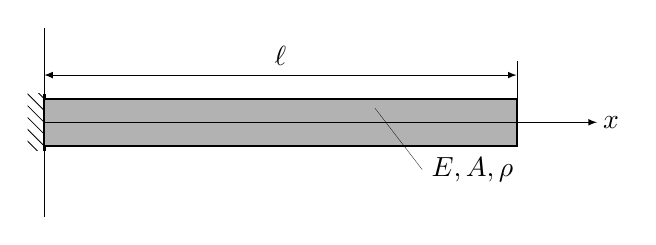
\begin{tikzpicture}[scale=0.6]
        \point{a}{0}{0};
        \support {3}{a}[270];

        % Draw the rectangle
        \filldraw[fill=gray!60, draw=black,thick] (0,-0.5) rectangle (10,0.5);

        %axis
        \draw[-latex, ultra thin] (0,0) -- (11.7,0);
        \draw[ultra thin] (0,-2) -- (0,2);
        \node at (12,0) {\(x\)};

        % length
        \draw[ultra thin] (10,0) -- (10, 1.3) ;
        \draw[latex-latex, ultra thin]  (0,1)  to node[sloped,midway,above] {$\ell$}(10,1) ;
        \draw[ultra thin]  (7,0.3) -- (8,-1) node[right]{$E,A,\rho$};
      \end{tikzpicture}
    \end{center}

    \column{0.5\textwidth}
    {\small \begin{itemize}
        \item $A$ cross-sectional area
        \item $\ell$ length
        \item $E$ Young's modulus
        \item $\rho$ material density
        \item $u_1$ axial displacement
        \item $x$ axial coordinate
      \end{itemize}}

  \end{columns}

  \vspace{0.5cm}
  \begin{block}{}
    \textbf{Objective:} find a Galerkin approximation of the axial displacement $u_{1}$ using appropriate functional spaces.
  \end{block}
\end{frame}

\begin{frame}{Galerkin approximation of longitudinal vibrations of a bar}
  Substituting
  $${\color{darkred} u_{1}^{h}(x,t)}=\mathbf H(x)\mathbf q(t)=\sum_{i=1}^nh_i(x)q_{i}(t)\quad\mbox{and}\quad {\color{orange}\delta u_{1}^{h}(x)}=\mathbf H(x)\bolddelta\mathbf q=\sum_{i=1}^nh_i(x)\delta q_{i}$$
  into the integral equation
  \[
    \int_0^\ell EA\, \partial_{x} {\color{darkred} u_1^h}\,\partial_{x}({\color{orange} \delta u_1^h})\ dx +\int_0^\ell\rho A {\color{darkred} \ddot{u}_1^h}{\color{orange} \delta u_1^h}\, dx=0,
  \]
  allow us to write
  \[
    \mathbf K\mathbf q(t)+\mathbf M\mathbf{\ddot q}(t)=0
  \]
  where
  \[
    k_{ij}  =\int_0^\ell EA\, h_i^\prime(x)h_j^\prime(x)\, dx, \qquad
    m_{ij}  =\int_0^\ell\rho A\, h_i(x)h_j(x)\, dx.
  \]
\end{frame}

\begin{frame}{Boundary and initial conditions}
  \begin{itemize}
    \item\textbf{Boundary conditions}:
          $$u_{1}^{h}(0,t)=0\quad\mbox{and}\quad \delta u_{1}^{h}(0,t)=0$$
          Therefore $\mathbf H(0)=\mathbf 0$.
          \vspace{0.5cm}\pause
    \item  \textbf{Initial conditions}:
          $$u_{1}^{h}(x,0)= u_{0}(x)\quad\mbox{and}\quad \dot u_{1}^{h}(x,0)= v_{0}(x)$$
          Thus $\mathbf q_{1}(0)=\mathbf q_{0}=\mathbf M^{-1}\int_\Omega \rho \mathbf H^T{u}_0\, d\Omega$ and $\mathbf{\dot q}_{1}(0)=\mathbf p_{0}=\mathbf M^{-1}\int_\Omega \rho \mathbf H^T{v}_0\, d\Omega$.
  \end{itemize}
\end{frame}

\begin{frame}{One-term Galerkin approximation}
  \begin{itemize}
    \item Let \textcolor{darkred}{$n=1$} then
          \begin{align*}
            u_{1}^{h}(x,t)      & =\mathbf H(x)\mathbf q(t)=h_{1}(x)q_{1}(t)            \\
            \delta u_{1}^{h}(x) & =\mathbf H(x)\bolddelta\mathbf q=h_{1}(x)\delta q_{1}
          \end{align*}
          where we choose
          $${\color{darkred} h_{1}(x)=\frac{x}{\ell}}.$$
          \emph{Notice that $h_{1}\in H^{1}(]0,\ell[)$ and $h_{1}(0)=0$.}
    \item The semi-discrete weak form is: find the function $q_{1}(t)$ such that:
          $$k_{11}q_{1}(t)+m_{11}\ddot q_{1}(t)=0$$
          $$k_{11}=\int_{0}^{\ell}EA \Big(\frac{1}{\ell}\Big)^{2}dx=\frac{EA}{\ell},\qquad m_{11}=\int_{0}^{\ell}\rho A \Big(\frac{x}{\ell}\Big)^{2}dx=\frac{\rho A\ell}{3}$$
  \end{itemize}
\end{frame}

{\setbeamercolor{background canvas}{bg=darkred!5}
\setbeamercolor{block body}{bg=darkred!5,fg=black}
\begin{frame}{Second order differential equation}
  \begin{block}{}
    The linear homogeneous second order ODE with constant coefficients governing the free vibration of single degree of
    freedom conservative system:
    $$\begin{cases}
        k_{11}q_{1}(t)+m_{11}\ddot q_{1}(t)=0 \\
        q_{1}(0)= q_{0}                       \\
        {\dot q}_{1}(0)= p_{0}
      \end{cases}$$
    admits an unique solution given by
    $$q_{1}(t)=p\cos(\omega_{1} t-\varphi),$$
    where the approx fundamental frequency is
    $$\omega_{1}=\sqrt{k_{11}/m_{11}}=\sqrt3\sqrt{E/\rho\ell^2},$$
    moreover $p=\sqrt{q_{0}^{2}+(p_{0}/\omega_1)^{2}}$ and $\tan(\varphi)=p_{0}/q_{0}\omega_1$.
  \end{block}
\end{frame}
}

\begin{frame}{Displacement approximation}
  \begin{block}{}
    $$u_1(x,t)=h_1(x)q_1(t)=\frac{p x}{\ell}\cos(\omega_{1} t-\varphi)$$
  \end{block}
  \begin{figure}
    \begin{subfigure}{.5\textwidth}
      \centering
      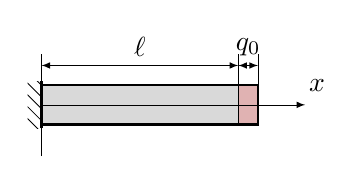
\begin{tikzpicture}[scale=0.5]
        \point{a}{0}{0};
        \support {3}{a}[270];
        % Draw the rectangle
        \filldraw[fill=gray!30] (0,-0.5) rectangle (5,0.5);
        \filldraw[fill=darkred!30] (5,-0.5) rectangle (5.5,0.5);
        \draw[draw=black,thick] (0,-0.5) rectangle (5.5,0.5);
        %axis
        \draw[-latex, ultra thin] (0,0) -- (6.7,0);
        \draw[ultra thin] (0,-1.3) -- (0,1.3);
        \node at (7,0.5) {\(x\)};
        % length
        \draw[ultra thin] (5,0) -- (5, 1.3) ;
        \draw[latex-latex, ultra thin]  (0,1)  to node[sloped,midway,above] {$\ell$}(5,1) ;
        \draw[ultra thin] (5.5,0) -- (5.5, 1.3) ;
        \draw[latex-latex, ultra thin]  (5,1)  to node[sloped,midway,above] {$q_0$}(5.5,1) ;
      \end{tikzpicture}
      \caption{$t=0$}
    \end{subfigure}%
    \begin{subfigure}{.5\textwidth}
      \centering
      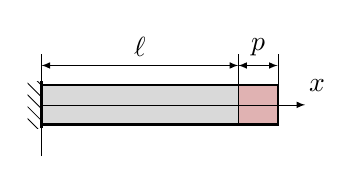
\begin{tikzpicture}[scale=0.5]
        \point{a}{0}{0};
        \support {3}{a}[270];
        % Draw the rectangle
        \filldraw[fill=gray!30] (0,-0.5) rectangle (5,0.5);
        \filldraw[fill=darkred!30] (5,-0.5) rectangle (6,0.5);
        \draw[draw=black,thick] (0,-0.5) rectangle (6,0.5);
        %axis
        \draw[-latex, ultra thin] (0,0) -- (6.7,0);
        \draw[ultra thin] (0,-1.3) -- (0,1.3);
        \node at (7,0.5) {\(x\)};
        % length
        \draw[ultra thin] (5,0) -- (5, 1.3) ;
        \draw[latex-latex, ultra thin]  (0,1)  to node[sloped,midway,above] {$\ell$}(5,1) ;
        \draw[ultra thin] (6,0) -- (6, 1.3) ;
        \draw[latex-latex, ultra thin]  (5,1)  to node[sloped,midway,above] {$p$}(6,1) ;
      \end{tikzpicture}
      \caption{$t=(\varphi+2k\pi)/\omega_1$}
    \end{subfigure}
    \vskip\baselineskip
    \begin{subfigure}{.5\textwidth}
      \centering
      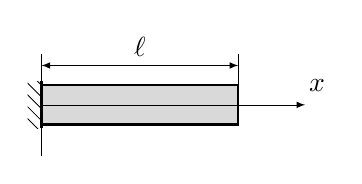
\begin{tikzpicture}[scale=0.5]
        \point{a}{0}{0};
        \support {3}{a}[270];
        % Draw the rectangle
        \filldraw[fill=gray!30, draw=black,thick] (0,-0.5) rectangle (5,0.5);
        %axis
        \draw[-latex, ultra thin] (0,0) -- (6.7,0);
        \draw[ultra thin] (0,-1.3) -- (0,1.3);
        \node at (7,0.5) {\(x\)};
        % length
        \draw[ultra thin] (5,0) -- (5, 1.3) ;
        \draw[latex-latex, ultra thin]  (0,1)  to node[sloped,midway,above] {$\ell$}(5,1) ;
      \end{tikzpicture}
      \caption{$t=(\varphi+\pi/2+k\pi)/\omega_1$}
    \end{subfigure}%
    \begin{subfigure}{.5\textwidth}
      \centering
      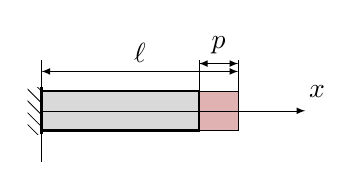
\begin{tikzpicture}[scale=0.5]
        \point{a}{0}{0};
        \support {3}{a}[270];
        % Draw the rectangle
        \filldraw[fill=gray!30] (0,-0.5) rectangle (5,0.5);
        \filldraw[fill=darkred!30] (4,-0.5) rectangle (5,0.5);
        \draw[draw=black,thick] (0,-0.5) rectangle (4,0.5);
        %axis
        \draw[-latex, ultra thin] (0,0) -- (6.7,0);
        \draw[ultra thin] (0,-1.3) -- (0,1.3);
        \node at (7,0.5) {\(x\)};
        % length
        \draw[ultra thin] (5,0) -- (5, 1.3) ;
        \draw[latex-latex, ultra thin]  (0,1)  to node[sloped,midway,above] {$\ell$}(5,1) ;
        \draw[ultra thin] (4,0) -- (4, 1.3) ;
        \draw[latex-latex, ultra thin]  (4,1.2)  to node[sloped,midway,above] {$p$}(5,1.2) ;
      \end{tikzpicture}
      \caption{$t=(\varphi+(2k+1)\pi)/\omega_1$}
    \end{subfigure}
  \end{figure}
\end{frame}

\begin{frame}{Fundamental frequency comparison}
  \begin{itemize}
    \item Approximated fundamental frequency: (obtained via one-term Galerkin)
          $$\omega_{1}=\sqrt{\frac{k_{11}}{m_{11}}}=\sqrt{3}\sqrt{\frac{E}{\rho \ell^{2}}}$$
    \item Exact fundamental frequency:
          $$\omega_{1}^{e}=\frac{\pi}{2}\sqrt{\frac{E}{\rho \ell^{2}}}$$
    \item Relative error:
          $$\mbox{relative error}=\frac{|\omega_{1}-\omega_{1}^{e}|}{\omega_{1}^{e}}=10.3\%$$
  \end{itemize}
\end{frame}

\begin{frame}{One-term quadratic Galerkin approximation}
  \begin{columns}[T]
    \begin{column}{.48\textwidth}\vspace{.7cm}
      Let $n=1$ and
      \begin{align*}
        u_{1}^{h}(x,t)      & =\mathbf H(x)\mathbf q(t)=h_{1}(x)q_{1}(t)            \\
        \delta u_{1}^{h}(x) & =\mathbf H(x)\bolddelta\mathbf q=h_{1}(x)\delta q_{1}
      \end{align*}
      where the shape function is choosen as
      $$\color{darkred}{h_{1}(x)=\frac{2x}{\ell}}\Big(1-\frac{x}{2\ell}\Big).$$
      Notice $h_{1}\in H^{1}(]0,\ell[)$ and $h_{1}(0)=0$.
    \end{column}
    \hfill
    \begin{column}{.5\textwidth}
      \begin{center}
        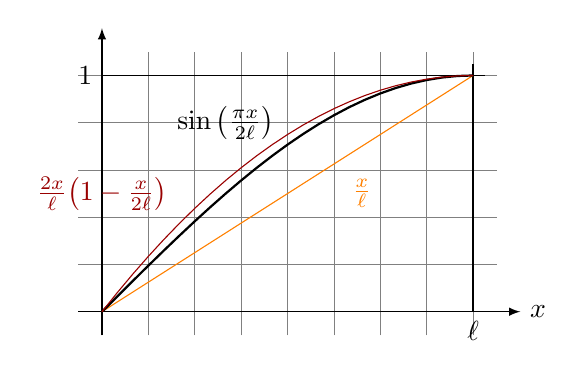
\begin{tikzpicture}[scale=3,domain=0:pi/2]
          \draw[very thin,color=gray,xstep=pi/16,ystep=0.2] (-0.1,-0.1) grid (pi/2+0.1,1.1);
          \draw[thin] (pi/2,0) node[below]{$\ell$} -- (pi/2,1.05);
          \draw[thin] (pi/2+0.05,1) -- (0, 1) node[left]{$1$};
          \draw[-latex] (-0.1,0) -- (pi/2+0.2,0) node[right] {$x$};
          \draw[-latex] (0,-0.1) -- (0,1.2);
          \draw[color=orange]    plot (\x,2/pi*\x);
          \draw[thick,color=black]   plot (\x,{sin(\x r)}) ;
          \draw[color=darkred] plot (\x,{4*\x/pi*(1-\x/pi)});
          \node at (pi/6,0.8)  {$\sin\big(\frac{\pi x}{2\ell}\big)$};
          \node[color=darkred] at (0,0.5)  {$\frac{2x}{\ell}\big(1-\frac{x}{2\ell}\big)$};
          \node[color=orange] at (1.1,0.5)  {$\frac{x}{\ell}$};
          % \x r means to convert '\x' from degrees to _r_adians:
        \end{tikzpicture}
      \end{center}
    \end{column}
  \end{columns}
\end{frame}

\begin{frame}{One-term quadratic Galerkin approximation}
  \begin{itemize}
    \item The stiffness and mass '\emph{matrices}' are
          \begin{align*}
            k_{11} & =\int_{0}^{\ell}\frac{4EA}{\ell^{2}}\Big(1-\frac{x}{\ell}\Big)^{2}dx=\frac{4EA}{3\ell}                  \\
            m_{11} & =\int_{0}^{\ell}\frac{4\rho A x^{2}}{\ell^{2}} \Big(1-\frac{x}{2\ell}\Big)^{2}dx=\frac{8\rho A\ell}{15}
          \end{align*}
    \item Approximated fundamental frequency: (obtained via one-term quadratic Galerkin)
          $$\omega_{1}=\sqrt{\frac{k_{11}}{m_{11}}}=\sqrt{\frac{5}{2}}\sqrt{\frac{E}{\rho \ell^{2}}}$$
    \item Relative error:
          $$\mbox{relative error}=\frac{|\omega_{1}-\omega_{1}^{e}|}{\omega_{1}^{e}}=0.7\%$$

  \end{itemize}
\end{frame}

\begin{frame}{$n$-terms Galerkin approximation}
  \begin{center}
    \href{https://drive.mathworks.com/sharing/6a9792ef-d0a7-4aca-a1d0-8b1862b0ac3b}{\beamergotobutton{Go to Matlab Drive}}
  \end{center}
\end{frame}

\begin{frame}{Advantages and drawbacks of Galerkin method}
  \textbf{In a nutshell:} Galerkin method transforms the partial differential equations (PDE), expressed in their weak formulation, into a system of ordinary differential equations (ODE).
  \vspace{0.7cm}
  \begin{columns}
    \begin{column}{0.5\textwidth}
      \textbf{Advantages:}
      \begin{itemize}
        \item[\Checkmark]Converges quickly with appropriate shape functions.
        \item[\Checkmark]  Provides a systematic and structured approach for approximating solutions.
        \item[\Checkmark] The same set of functions is used to express real and virtual variables.
      \end{itemize}
    \end{column}

    \begin{column}{0.5\textwidth}
      \textbf{Drawbacks:}
      \begin{itemize}
        \item[\XSolidBrush] Accuracy heavily dependent on choice of basis functions.
        \item[\XSolidBrush]No physical interpretation of the unknown variable $\mathbf q(t)$.
        \item[\XSolidBrush] The formulation of initial and boundary conditions in the discretized form is cumbersome.
      \end{itemize}
    \end{column}
  \end{columns}
\end{frame}

\section{Finite element method in global coordinate system}

\begin{frame}{Divide and conquer mentality}
  \begin{itemize}
    \item The geometry of a structure is discretised when it is split into a mesh of finite elements ${}^1\Omega,\dots,{}^m\Omega$ (smaller components or regular shapes).
    \item The discretisation introduces an approximation error which can be reduced by using a finer mesh (i.e. more elements), or by increasing the accuracy of the finite elements chosen.
    \item Discretisation starts with the definition of a \textbf{set of nodes}: $\mathbf x_i$, $i=1,\dots, p$.
  \end{itemize}
  \begin{center}
    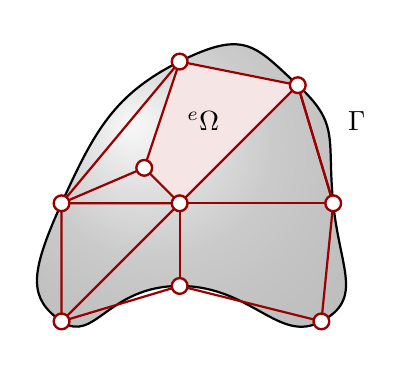
\begin{tikzpicture}[scale=1.5]
      %\draw[step=1.0,black,thin] (0,0) grid (4,4);
      % Draw the potato-like shape
      \shade [ball color= gray!90!black, opacity=.3] plot [thick,smooth cycle, tension=1] coordinates  {(1,2) (2,3.2) (3,3) (3.3,2) (3.2,1) (2,1.3) (1,1)};
      \draw[thick] plot [thick,smooth cycle, tension=1] coordinates {(1,2) (2,3.2) (3,3) (3.3,2) (3.2,1) (2,1.3) (1,1)};
      \draw[fill=darkred!30,thick,darkred!10] (2,2) -- (3,3) -- (2,3.2) -- (1.7,2.3) -- cycle;
      % Label the region Omega	
      \node at (2.2,2.7) {${}^e\Omega$};
      % Label the boundary Gamma
      \node at (3.5,2.7) {$\Gamma$};
      \draw[thick,darkred] (1,2) -- (2,3.2) -- (3,3) -- (3.3,2) -- (3.2,1) -- (2,1.3) -- (1,1) -- cycle;
      \draw[thick,darkred] (1,2) -- (2,2) -- (3,3) -- (3.3,2);
      \draw[thick,darkred] (2,1.3) -- (2,2) -- (3.3,2);
      \draw[thick,darkred] (1,1) -- (2,2) -- (1.7,2.3) -- (2,3.2);
      \draw[thick,darkred] (1.7,2.3) -- (1,2);
      \node[darkred,draw,shape=circle,fill=white,minimum size=2mm,line width=0.3mm,inner sep=0] at (1,1) {};
      \node[darkred,draw,shape=circle,fill=white,minimum size=2mm,line width=0.3mm,inner sep=0] at (1,2) {};
      \node[darkred,draw,shape=circle,fill=white,minimum size=2mm,line width=0.3mm,inner sep=0] at (2,2) {};
      \node[darkred,draw,shape=circle,fill=white,minimum size=2mm,line width=0.3mm,inner sep=0] at (2,1.3) {};
      \node[darkred,draw,shape=circle,fill=white,minimum size=2mm,line width=0.3mm,inner sep=0] at (2,3.2) {};
      \node[darkred,draw,shape=circle,fill=white,minimum size=2mm,line width=0.3mm,inner sep=0] at (1.7,2.3) {};
      \node[darkred,draw,shape=circle,fill=white,minimum size=2mm,line width=0.3mm,inner sep=0] at (3,3) {};
      \node[darkred,draw,shape=circle,fill=white,minimum size=2mm,line width=0.3mm,inner sep=0] at (3.2,1) {};
      \node[darkred,draw,shape=circle,fill=white,minimum size=2mm,line width=0.3mm,inner sep=0] at (3.3,2) {};
    \end{tikzpicture}
  \end{center}
\end{frame}

\begin{frame}{Nodes, elements and shape functions}
  \begin{center}
    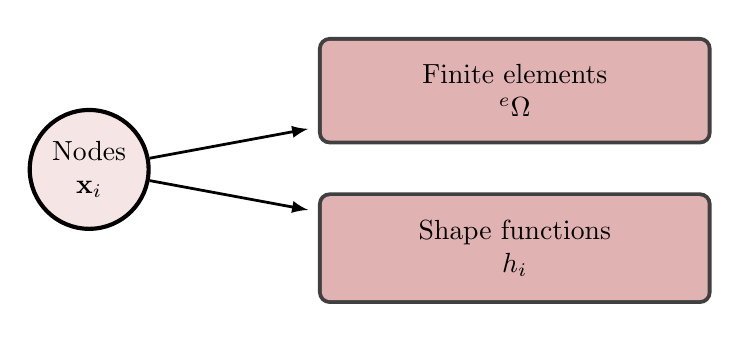
\begin{tikzpicture}[node distance=2cm,>=stealth,thick]
      % Define nodes
      \node (Nodes) [circle, draw, minimum size=1.5cm, align=center, fill=darkred!10,line width=1.5pt] {Nodes\\ $\mathbf x_i$};

      \node (Elem) [right=of Nodes, yshift=+1cm]  {
        \begin{tcolorbox}[colback=darkred!30, width=5cm]
          \centering Finite elements \\ $\mathbf {}^e\Omega$
        \end{tcolorbox}
      };

      \node (Func) [right=of Nodes, yshift=-1cm]  {
        \begin{tcolorbox}[colback=darkred!30, width=5cm]
          \centering Shape functions\\ $h_i$
        \end{tcolorbox}
      };

      % Draw arrows
      \draw[-latex,line width=1pt] (Nodes) -- (Elem);
      \draw[-latex,line width=1pt] (Nodes) -- (Func);
    \end{tikzpicture}
  \end{center}
  \begin{itemize}
    \item \textbf{Finite element method:} a special case of the Galerkin method, where shape functions are systematically defined in terms of nodes.
    \item Each shape function is non-zero only on a very limited number of finite elements (\emph{compact support}).
    \item The computation of the mass and stiffness matrix is enhanced by the local nature of the shape functions.
  \end{itemize}
\end{frame}

{\setbeamercolor{background canvas}{bg=darkred}
\setbeamercolor{block body}{bg=darkred,fg=white}
\setbeamercolor{itemize item}{fg=white}
\begin{frame}{Displacements approximation}
  \begin{block}{}
    Let $p$ the number of nodes of the mesh.
    \vspace{-.2cm}
    \begin{align*}
      \mathbf u^{h}(\mathbf x,t)     & =\mathbf H(\mathbf x)\mathbf q(t)    \\
      \delta\mathbf u^{h}(\mathbf x) & =\mathbf H(\mathbf x)\delta\mathbf q
    \end{align*}
    \vspace{-.8cm}
    \begin{itemize}
      \item $\mathbf H(\mathbf x)$ is a $3\times 3p$ matrix of \textbf{shape functions}.
            $$
              \mathbf H
              =\left[
                \begin{array}{c;{2pt/2pt}c;{2pt/2pt}c;{2pt/2pt}c;{2pt/2pt}c;{2pt/2pt}c}
                  h_{1}\mathbf I & h_{2}\mathbf I & \dots & h_{i}\mathbf I & \dots & h_{p}\mathbf I \\
                \end{array} \right]
            $$
            $\mathbf I$ is the $3\times 3$ identity matrix.
      \item $\mathbf q(t)$ is a $3p\times 1$ vector of (\emph{unknown}) time-dependent functions.
      \item $\delta \mathbf q$ is a $3p\times 1$ vector of constants.
    \end{itemize}


  \end{block}
\end{frame}
}

\begin{frame}{Displacements approximation - matrix notation}
  \begin{block}{}
    {\small
      $$\begin{pmatrix}
          u_{1}^{h} \\
          u_{2}^{h} \\
          u_{3}^{h} \\
        \end{pmatrix}
        =
        \left[
          \begin{array}{ccc;{2pt/2pt}ccc;{2pt/2pt}c;{2pt/2pt}ccc}
            h_{1} & 0     & 0     & h_{2} & 0     & 0     &       & h_{p} & 0     & 0     \\
            0     & h_{1} & 0     & 0     & h_{2} & 0     & \dots & 0     & h_{p} & 0     \\
            0     & 0     & h_{1} & 0     & 0     & h_{2} &       & 0     & 0     & h_{p} \\
          \end{array} \right]
        \begin{pmatrix}
          q_{1,1} \\
          q_{1,2} \\
          q_{1,3} \\
          \vdots  \\
          q_{p,1} \\
          q_{p,2} \\
          q_{p,3} \\
        \end{pmatrix}
      $$

      $$\begin{pmatrix}
          \delta u_{1}^{h} \\
          \delta u_{2}^{h} \\
          \delta u_{3}^{h} \\
        \end{pmatrix}
        =
        \left[
          \begin{array}{ccc;{2pt/2pt}ccc;{2pt/2pt}c;{2pt/2pt}ccc}
            h_{1} & 0     & 0     & h_{2} & 0     & 0     &       & h_{p} & 0     & 0     \\
            0     & h_{1} & 0     & 0     & h_{2} & 0     & \dots & 0     & h_{p} & 0     \\
            0     & 0     & h_{1} & 0     & 0     & h_{2} &       & 0     & 0     & h_{p} \\
          \end{array} \right]
        \begin{pmatrix}
          \delta  q_{1,1} \\
          \delta q_{1,2}  \\
          \delta q_{1,3}  \\
          \vdots          \\
          \delta  q_{p,1} \\
          \delta q_{p,2}  \\
          \delta q_{p,3}  \\
        \end{pmatrix}
      $$
    }
  \end{block}
\end{frame}

\begin{frame}{Displacements approximation - index notation}
  \begin{block}{}
    \vspace{-.5cm}
    \begin{align*}
      \mathbf u^{h}(\mathbf x,t)=\sum_{i=1}^{p}h_{i}(\mathbf x)\mathbf q_{i}(t) \\
      \boldsymbol\delta \mathbf u^{h}(\mathbf x,t)=\sum_{i=1}^{p}h_{i}(\mathbf x)\bolddelta\mathbf q_{i}
    \end{align*}
    {\small
    $$\mathbf q_i(t)=\begin{pmatrix}
        q_{i,1}(t) \\
        q_{i,2}(t) \\
        q_{i,3}(t) \\
      \end{pmatrix}\qquad \mbox{and} \qquad
      \bolddelta\mathbf q_{i}=\begin{pmatrix}
        \delta q_{i,1} \\
        \delta q_{i,2} \\
        \delta q_{i,3} \\
      \end{pmatrix}
    $$
    }
  \end{block}
\end{frame}

\begin{frame}{Deformation, stiffness, mass matrices and loads vector}
  \begin{itemize}
    \item $\mathbf B=\boldsymbol\nabla\mathbf H$ is a ($6\times 3p$) matrix:
          \begin{align*}
            \mathbf B
            =\left[
              \begin{array}{ccc;{2pt/2pt}c;{2pt/2pt}ccc}
                \partial_xh_{1} & 0               & 0               &       & \partial_xh_{p} & 0               & 0               \\
                0               & \partial_yh_{1} & 0               & \dots & 0               & \partial_yh_{p} & 0               \\
                0               & 0               & \partial_zh_{1} &       &
                0               & 0               & \partial_zh_{p}                                                               \\
                0               & \partial_zh_{1} & \partial_yh_{1} &       &
                0               & \partial_zh_{p} & \partial_yh_{p}                                                               \\
                \partial_zh_{1} & 0               & \partial_xh_{1} & \dots & \partial_zh_{p} & 0               & \partial_xh_{p} \\
                \partial_yh_{1} & \partial_xh_{1} & 0               &       & \partial_yh_{p} & \partial_xh_{p} & 0               \\
              \end{array} \right]
            =\left[
              \begin{array}{c;{2pt/2pt}c;{2pt/2pt}c}
                \boldsymbol\nabla h_1 & \dots & \boldsymbol\nabla h_p
              \end{array} \right]
          \end{align*}
          \vspace{0.1cm}
    \item $\mathbf K$ and $\mathbf M$ are ($3p\times 3p$) matrices and $\mathbf r$ is a ($3p\times 1$) vector:
          \[
            \mathbf K =\int_\Omega \mathbf B^T\mathbf C\mathbf B \, d\Omega,\qquad \mathbf M =\int_\Omega \rho\, \mathbf H^T\mathbf H \, d\Omega,\qquad \mathbf r(t)=\int_{\Gamma_\sigma} \mathbf H^{T}\mathbf{\hat f} \, d\Gamma+\int_{\Omega} \mathbf H^{T}\mathbf f\, d\Omega.
          \]
  \end{itemize}
\end{frame}

\begin{frame}{Global nodal shape functions - construction guidelines}
  Global nodal shape functions \( h_i: \Omega \to \mathbb R \) are characterized by the following properties:
  \vspace{0.3cm}
  \begin{itemize}
    \item They form a linearly independent basis of polynomials of a given degree.
    \item Their values lie in the interval \( [0,1] \).
    \item They satisfy the Kronecker delta property:
          \[ h_i(\mathbf{x}_j) = \delta_{ij} = \begin{cases}
              1 & \text{if } i = j    \\
              0 & \text{if } i \neq j
            \end{cases}
          \]
    \item The functions \( h_i \) vanish on all finite elements that are not adjacent to the node \( \mathbf{x}_i \).
  \end{itemize}
\end{frame}

{\setbeamercolor{background canvas}{bg=darkred}
\setbeamercolor{block body}{bg=darkred,fg=white}
\setbeamercolor{itemize item}{fg=white}
\begin{frame}{Properties of shape functions - convergence criteria}
  \begin{block}{}
    \begin{itemize}
      \item Continuity of $h_i$ at nodes and interfaces of finite elements.
      \item Differentiability of $h_i$ inside each finite element.
      \item Completeness (rigid body motion and constant deformation):
            $$\sum_{i=1}^{p}h_{i}(\mathbf x)=1 \quad\text{and}\quad \sum_{i=1}^{p}\boldsymbol\nabla h_{i}(\mathbf x)=\mathbf 0.$$
      \item Approximate real and virtual diplacements at the nodes:
            \begin{align*}
              \mathbf u^h(\mathbf x_j,t)         & =\sum_{i=1}^{p}h_{i}(\mathbf x_j)\mathbf q_{i}(t)=\mathbf q_j(t),               \\
              \bolddelta\mathbf u^h(\mathbf x_j) & =\sum_{i=1}^{p}h_{i}(\mathbf x_j)\bolddelta\mathbf q_{i}=\bolddelta\mathbf q_j.
            \end{align*}
    \end{itemize}
  \end{block}
\end{frame}
}

\begin{frame}{Treatment of boundary conditions}
  On $\Gamma_{u}$ we impose $\mathbf u^{h}=\mathbf{\hat u}$ and $\bolddelta\mathbf u^{h}=\mathbf 0$. Consequently for every node $\mathbf x_j\in\Gamma_u$:
  $$\mathbf q_j(t)=\mathbf u^h(\mathbf x_j,t)=\mathbf{\hat u}(\mathbf x_j,t)\quad\mbox{ and }\qquad \bolddelta\mathbf q_j=\bolddelta\mathbf u^h(\mathbf x_j,t)=\mathbf 0.$$
  \begin{center}
    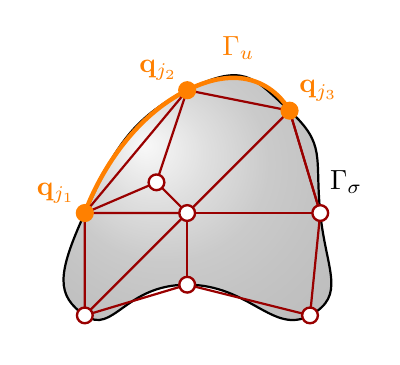
\begin{tikzpicture}[scale=1.3]
      %\draw[step=1.0,black,thin] (0,0) grid (4,4);
      % Draw the potato-like shape
      \shade [ball color= gray!90!black, opacity=.3] plot [thick,smooth cycle, tension=1] coordinates  {(1,2) (2,3.2) (3,3) (3.3,2) (3.2,1) (2,1.3) (1,1)};
      \draw[thick] plot [thick,smooth cycle, tension=1] coordinates {(1,2) (2,3.2) (3,3) (3.3,2) (3.2,1) (2,1.3) (1,1)};
      % Boundary 
      \draw[ultra thick, orange] plot [smooth, tension=1.3] coordinates {(1,2) (2,3.2) (3,3)};
      \node[orange, above] at (2.5,3.4) {$\Gamma_u$};
      \node[right] at (3.3,2.3) {$\Gamma_\sigma$};
      % Finite elements 
      \draw[thick,darkred] (1,2) -- (2,3.2) -- (3,3) -- (3.3,2) -- (3.2,1) -- (2,1.3) -- (1,1) -- cycle;
      \draw[thick,darkred] (1,2) -- (2,2) -- (3,3) -- (3.3,2);
      \draw[thick,darkred] (2,1.3) -- (2,2) -- (3.3,2);
      \draw[thick,darkred] (1,1) -- (2,2) -- (1.7,2.3) -- (2,3.2);
      \draw[thick,darkred] (1.7,2.3) -- (1,2);
      \node[darkred,draw,shape=circle,fill=white,minimum size=2mm,line width=0.3mm,inner sep=0] at (1,1) {};
      \node[orange,draw,shape=circle,fill=orange,minimum size=2mm,line width=0.3mm,inner sep=0] at (1,2) {};
      \node[orange,above left] at (1,2) {$\mathbf q_{j_1}$};
      \node[darkred,draw,shape=circle,fill=white,minimum size=2mm,line width=0.3mm,inner sep=0] at (2,2) {};
      \node[darkred,draw,shape=circle,fill=white,minimum size=2mm,line width=0.3mm,inner sep=0] at (2,1.3) {};
      \node[orange,draw,shape=circle,fill=orange,minimum size=2mm,line width=0.3mm,inner sep=0] at (2,3.2) {};
      \node[orange,above left] at (2,3.2) {$\mathbf q_{j_2}$};
      \node[darkred,draw,shape=circle,fill=white,minimum size=2mm,line width=0.3mm,inner sep=0] at (1.7,2.3) {};
      \node[orange,draw,shape=circle,fill=orange,minimum size=2mm,line width=0.3mm,inner sep=0] at (3,3) {};
      \node[orange,above right] at (3,3) {$\mathbf q_{j_3}$};
      \node[darkred,draw,shape=circle,fill=white,minimum size=2mm,line width=0.3mm,inner sep=0] at (3.2,1) {};
      \node[darkred,draw,shape=circle,fill=white,minimum size=2mm,line width=0.3mm,inner sep=0] at (3.3,2) {};
    \end{tikzpicture}
  \end{center}
  \begin{itemize}
    \item[\Checkmark]
          The $j$-th component of the approximated nodal displacement $\mathbf{q}$ is know for every node $\mathbf x_j\in\Gamma_u$.
  \end{itemize}
\end{frame}

\begin{frame}{Treatment of initial conditions}
  Since \( \mathbf{u}(\mathbf{x},0) = \mathbf{u}_0(\mathbf{x}) \), enforcing \( \mathbf{u}^h(\mathbf{x},0) = \mathbf{u}_0(\mathbf{x}) \) ensures that the approximate displacement field is consistent with the initial condition. This leads to
  \[
    \mathbf{q}_j(0) = \mathbf{u}^h(\mathbf{x}_j,0) = \mathbf{u}_0(\mathbf{x}_j).
  \]
  Similarly, imposing the initial velocity condition, $ \dot{\mathbf{u}}(\mathbf{x},0) = \mathbf{v}_0(\mathbf{x})$, gives
  \[
    \mathbf{\dot{q}}_j(0) = \mathbf{\dot{u}}^h(\mathbf{x}_j,0) = \mathbf{v}_0(\mathbf{x}_j).
  \]
  \vspace{-0.5cm}
  \begin{itemize}
    \item[\Checkmark]
          These expressions provide the initial values of the unknown vector \( \mathbf{q} \) directly in terms of the given initial data \( \mathbf{u}_0 \) and \( \mathbf{v}_0 \).
  \end{itemize}
\end{frame}


\begin{frame}{Advantages and drawbacks of finite element method}
  \begin{columns}
    \begin{column}{0.5\textwidth}
      \textbf{Advantages:}
      \begin{itemize}
        \item[\Checkmark] Versatile for various engineering problems: mechanics of solids and fluids, dynamics, heat transfer, electrostatics, and more.
        \item[\Checkmark] Provides a systematic algorithm: defines the underlying shape functions used in the approximation.
        \item[\Checkmark]  Accuracy control: solution precision can be improved by refining the mesh.
      \end{itemize}
    \end{column}

    \begin{column}{0.5\textwidth}
      \textbf{Drawbacks:}
      \begin{itemize}
        \item[\XSolidBrush]Choice of mathematical model is crucial: the solution's reliability hinges on selecting an appropriate model.
        \item[\XSolidBrush]Computational cost: highly refined models increase the computational burden.
        \item[\XSolidBrush]Requires experience in meshing, boundary conditions, and solver settings.
      \end{itemize}
    \end{column}
  \end{columns}
\end{frame}


\end{document}